%%%%%%%%%%%%%%%%%%%%%%%%%%%%%%%%%%%%%%%%%%%%%%%%%%%%%%%%%%%%%%%%%%%%%%%%%%%%%%%%
%%%%%%%%%%%%%%%%%%   Vorlage für eine Abschlussarbeit   %%%%%%%%%%%%%%%%%%%%%%%%
%%%%%%%%%%%%%%%%%%%%%%%%%%%%%%%%%%%%%%%%%%%%%%%%%%%%%%%%%%%%%%%%%%%%%%%%%%%%%%%%

% Erstellt von Maximilian Nöthe, <maximilian.noethe@tu-dortmund.de>
% ausgelegt für lualatex und Biblatex mit biber

% Kompilieren mit
% latexmk --lualatex --output-directory=build thesis.tex
% oder einfach mit:
% make

\documentclass[
  %tucolor,       % remove for less green,
  BCOR=12mm,     % 12mm binding corrections, adjust to fit your binding
  parskip=half,  % new paragraphs start with half line vertical space
  open=any,      % chapters start on both odd and even pages
  cleardoublepage=plain,  % no header/footer on blank pages
]{tudothesis}


% Warning, if another latex run is needed
\usepackage[aux]{rerunfilecheck}

% just list chapters and sections in the toc, not subsections or smaller
\setcounter{tocdepth}{1}

%------------------------------------------------------------------------------
%------------------------------ Fonts, Unicode, Language ----------------------
%------------------------------------------------------------------------------
\usepackage{fontspec}
\defaultfontfeatures{Ligatures=TeX}  % -- becomes en-dash etc.

% german language
\usepackage{polyglossia}
\setdefaultlanguage{german}

% for english abstract and english titles in the toc
\setotherlanguages{english}

% intelligent quotation marks, language and nesting sensitive
\usepackage[autostyle]{csquotes}

% microtypographical features, makes the text look nicer on the small scale
\usepackage{microtype}

%------------------------------------------------------------------------------
%------------------------ Math Packages and settings --------------------------
%------------------------------------------------------------------------------

\usepackage{amsmath}
\usepackage{amssymb}
\usepackage{mathtools}

% Enable Unicode-Math and follow the ISO-Standards for typesetting math
\usepackage[
  math-style=ISO,
  bold-style=ISO,
  sans-style=italic,
  nabla=upright,
  partial=upright,
]{unicode-math}
\setmathfont{Latin Modern Math}

% nice, small fracs for the text with \sfrac{}{}
\usepackage{xfrac}


%------------------------------------------------------------------------------
%---------------------------- Numbers and Units -------------------------------
%------------------------------------------------------------------------------

\usepackage[
  locale=DE,
  separate-uncertainty=true,
  per-mode=symbol-or-fraction,
]{siunitx}
\sisetup{math-micro=\text{µ},text-micro=µ}

%------------------------------------------------------------------------------
%-------------------------------- tables  -------------------------------------
%------------------------------------------------------------------------------

\usepackage{booktabs}       % \toprule, \midrule, \bottomrule, etc

%------------------------------------------------------------------------------
%-------------------------------- graphics -------------------------------------
%------------------------------------------------------------------------------

\usepackage{graphicx}
\usepackage{grffile}
% allow figures to be placed in the running text by default:
\usepackage{scrhack}
\usepackage{float}
\floatplacement{figure}{htbp}
\floatplacement{table}{htbp}

% keep figures and tables in the section
\usepackage[section, below]{placeins}


%------------------------------------------------------------------------------
%---------------------- customize list environments ---------------------------
%------------------------------------------------------------------------------

\usepackage{enumitem}

%------------------------------------------------------------------------------
%------------------------------ Bibliographie ---------------------------------
%------------------------------------------------------------------------------

\usepackage[
  backend=biber,   % use modern biber backend
  autolang=hyphen, % load hyphenation rules for if language of bibentry is not
                   % german, has to be loaded with \setotherlanguages
                   % in the references.bib use langid={en} for english sources
  sorting=none,
]{biblatex}
\addbibresource{references.bib}  % the bib file to use

\DefineBibliographyStrings{german}{andothers = {{et\,al\adddot}}}  % replace u.a. with et al.
\usepackage{bibstyle}
\usepackage{emptypage}
% Last packages, do not change order or insert new packages after these ones
\usepackage[pdfusetitle, unicode, linkbordercolor=tugreen]{hyperref}
\usepackage{bookmark}
\usepackage[shortcuts]{extdash}

%------------------------------------------------------------------------------
%-------------------------    Angaben zur Arbeit   ----------------------------
%------------------------------------------------------------------------------

\author{Christopher Krause}
\title{Entwicklung eines Programmes zur Berechnung von Annealingeffekten in bestrahltem Silizium nach dem Hamburger Modell}
\date{2019}
\birthplace{Mainz}
\chair{Lehrstuhl für Experimentelle Physik IV}
\division{Fakultät Physik}
\thesisclass{Bachelor of Science}
\submissiondate{12. Juli 2019}
\firstcorrector{Dr.~Jens Weingarten}
\secondcorrector{Prof.~Dr.~Dr.~Wolfgang Rhode}

% tu logo on top of the titlepage
\titlehead{\includegraphics[height=1.5cm]{logos/tu-logo.pdf}}

\begin{document}
\frontmatter
%\thispagestyle{empty}
\setcounter{page}{2}
\section*{Hinweise}
Empfohlen wird die Verwendung dieser Vorlage mit der jeweils aktuellsten TeXLive Version (Linux, Windows) bzw. MacTeX Version (MacOS).
Aktuell ist dies TeXLive 2016. Download hier:
\begin{center}
  \ttfamily\url{https://www.tug.org/texlive/}
\end{center}
Bei Verwendung von TexLive Versionen 2014 und älter sollte
die Zeile
\begin{center}
\verb+\RequirePackage{fixltx2e}+ 
\end{center}
als erste Zeile der Präambel noch vor der Dokumentenklasse eingefügt werden.
Dies lädt diverse Bugfixes für LaTeX, die ab TexLive 2015 Standard sind.

Die Vorlage \texttt{thesis.tex} ist für die Kompilierung mit \texttt{lualatex} ausgelegt, mit wenigen Anpassungen kann sie aber auch mit \texttt{pdflatex} oder \texttt{xelatex} verwendet werden. 
Die Dokumentenklasse \texttt{tudothesis.cls} kann mit allen drei Programmen verwednet werden.

Achten Sie auch auf die Kodierung der Quelldateien.
Bei Verwendung von Xe\LaTeX\ oder Lua\LaTeX\ (empfohlen) müssen die
Quelldateien UTF-8 kodiert sein.
Bei Verwendung von pdf\LaTeX\ nutzen Sie die Pakete \texttt{inputenc} und \texttt{fontenc} mit der korrekten Wahl der Kodierungen.

Eine aktuelle Version dieser Vorlage steht unter 
\begin{center}
  \ttfamily\url{https://github.com/maxnoe/tudothesis}
\end{center}
zur Verfügung.

Alle verwendeten Pakete werden im \LaTeX{} Kurs von Pep et al.\ erklärt:
\begin{center}
  \ttfamily\url{http://toolbox.pep-dortmund.org/notes}
\end{center}

Für Rückmeldungen und bei Problemen mit der Klasse oder Vorlage, bitte ein \emph{Issue} auf GitHub aufmachen oder eine Email an
\href{mailto:maximilian.noethe@tu-dortmund.de}{maximilian.noethe@tu-dortmund.de} schreiben.

Wenn Sie die Dokumentenklasse mit der Option \texttt{tucolor} laden, werden verschiedene Elemente in TU-Grün gesetzt.

\maketitle

% Gutachterseite
\makecorrectorpage

% hier beginnt der Vorspann, nummeriert in römischen Zahlen
\thispagestyle{plain}

\section*{Kurzfassung}
Hier steht eine Kurzfassung der Arbeit in deutscher Sprache inklusive der Zusammenfassung der
Ergebnisse.
Zusammen mit der englischen Zusammenfassung muss sie auf diese Seite passen.

\section*{Abstract}
\begin{english}
The abstract is a short summary of the thesis in English, together with the German summary it has to fit on this page.
\end{english}

\tableofcontents

\mainmatter
% Hier beginnt der Inhalt mit Seite 1 in arabischen Ziffern
\chapter{Einleitung}
Siliziumdetektoren sind in der Hochenergiephysik und in der Industrie weit verbreitete
Detektoren, welche in Collider-Experimenten, wie Atlas, verwendet werden.
Sie operieren bei Raumtemperatur und können präzise Rückschlüsse auf die
Energie von Teilchen schließen. Einfallende Teilchen können die
Struktur des Detektors verändern, wodurch dieser ineffizienter wird.
Es ist somit notwendig, die Strahlenschäden möglichst gering zu halten damit
die Halbleiter eine möglichst lange Lebenszeit besitzen. Manche Schäden sind durch annealing nicht
aufhebbar, wodurch die Detektoren unweigerlich mit fortlaufendem Einsatz
an Leistungsfähigkeit verlieren. Um die reparablen Schäden im Siliziumkristall
zu beseitigen wird der Annealingeffekt genutzt. Hierbei wird durch zugeführte Wärme gewisse
Defekte entfernt.
Zusätzlich sorgt die Bestrahlung der Detekoren für einen anwachsenden Leckstrom, welcher den
gemessenen elektrischen Signalen überlagert ist und ein Rauschen kreiert. Ein
effektiver Detektor sollte somit einen möglichst geringen Leckstrom haben.
Für einen Detektor ist eine möglichst große Depletionszone ebenfalls wichtig, idealerweise
liegt eine vollständige Depletion des Detekorvolumens vor. Um dies zu erreichen wird
eine externe Spannung verwendet. Mit steigender Spannung wächst jedoch auch der Leckstrom, weshalb
darauf geachtet werden muss bei möglichst geringer externer Spannung den Detektor zu depletieren.
Dies ist abhängig von der Dotierungskonzentration, da sie die Ladung der
Raumladungszone beschreibt.

Die durch Strahlung induzierte Änderung der Dotierungskonzentration und des Leckstromes sind
somit wichtige Größen für die Qualität eines Detektors. In dieser Arbeit wird das
theoretische Verhalten der beiden Größen auf der Grundlage des Hamburger-Modells betrachtet.
Ein Programm zur Modellierung von Annealingeffekten kann somit zur
optimierung des Annealingprozesses beitragen.


Das oben erwähnte Collider-Experiment, ATLAS, verwendet Siliziumdetekoren als
einen Teil seines inneren Detektors zur Bestimmung von Richtung, Impuls
und Ladung von geladenen Teilchen. Es ist Teil des LHC am Cern und umfasst
das größte Volumen aller Detektoren, die bisher gebaut wurden\cite{atlas}.
Der innere Detektor ist zylinderförmig mit einer Länge von $\SI{6.2}{\meter}$ und
einem Radius von $\SI{2.1}{\meter}$. Er wird von einem $\SI{2}{\tesla}$ Magnetfeld
durchsetzt und kann Teilchen mit geringen Energien von $\SI{0.5}{\giga\eV}$ noch detektieren.
Bestehend aus drei Komponenenten, dem Pixeldetektor, dem "Semiconductor Tracker" (SCT) und dem "Transition Radiation Tracker" (TCT) kommen  die
Siliziumdetektoren in allen drei Bestandteilen zum Einsatz.
Mit einer Fläche von $\SI{1.7}{\meter\squared}$, drei Lagen und insgesamt 1744 Modulen ist es möglich
Information über die Strecke der entstehenden Teilchen zu erlangen. Der SCT besteht aus 4088 Modulen über vier zylindrische Lagen,
sowie 18 scheibenförmige Lagen, verteilt und umfasst eine Fläche von $\SI{63}{\meter\squared}$. Auch dieser wird für
die Rekonstruktion der Bahn der Teilchen verwendet, jedoch auch für die Identifikation und der Bestimmung des Impulses der Teilchen.
Der TCT wird ebenfalls zur Identifikation von Teilchen, hauptsächlich Elektronen und Pionen, verwendet und besteht aus 73 Lagen
von Straw-Detektoren (viele aneinander gereihte Proportionalzählrohre).

\chapter{Theoretische Grundlagen}


\section{Siliziumdetektoren}

Die im Halbleiter vorkommenden Elektronen des Siliziumkristalls wechselwirken mit anderen Elektronen und
Kernen, wodurch es zu vielen Aufspaltungen des Energieniveaus dieser kommt. Die
Zustände liegen dicht bei einander, weshalb von Energiebändern gesprochen wird.
Das höchste von den Elektronen besetzte Band ist das Valenzband, welches von dem
nächsthöheren Band durch eine Bandlücke getrennt ist. Elektronen können
durch Anregungen in das Leitungsband wandern und somit Strom leiten, vorausgesetzt
die Anregungen sind größer als die Energielücke.

Das Einbringen von Fremdatomen in den Siliziumkristall kann dessen Eigenschaften ändern
und wird Dotierung genannt.
Hat das Fremdatom mehr oder weniger Valenzelektronen als das Silizium, kommt
es zu weiteren Aufspaltungen der Energieniveaus, welche sich in der Energielücke
befindet. Dadurch wird es für Elektronen einfacher in das Leitungsband zu wandern.
Bei den Fremdatomen wird zwischen Donatoren und Akzeptoren unterschieden, wobei die
Ersteren mehr Valenzelektronen als das Silizium besitzen und die Zweiteren weniger.
Bereiche des Siliziumkristalls mit Donatoren werden n-Dotierte Halbleiter
und Bereiche mit Akzeptoren p-Dotierte Halbleiter genannt.

Bei einem Übergang von einer n-Dotierten zu einer p-Dotierten Schicht rekombinieren
die Elektronen der n-Dotierten Schicht mit den Elektronenlöchern der p-dotierten Schicht, da beide
in die anderen Bereiche diffundieren. Durch die übrig bleibenden ortsfesten Atomkerne
baut sich ein elektrisches Feld auf, welches dem Diffusionsstrom entgegenwirkt.
Ein sich einstellendes Gleichgewicht führt zu einer raumladungsfreien Zone bei
dem p-n-Übergang.
Für Detektoren werden die eiden Schichten unterschiedlich stark Dotiert, wobei typischerweise
mehr Akzeptoren als Donatoren in den Siliziumkristall eingebracht werden. Bei
asymmetrischer Dotierung breitet sich die Depletionszone hauptsächlich in die schwächer dotierte Seite aus.
Mit dieser Annahme ($N_{\mathrm{A}} \gg N_{\mathrm{D}}$) lässt sich die Depletionstiefe $d$ beschreiben durch:
\begin{align}
  d \approx \sqrt{\frac{2 \epsilon \epsilon_0}{e} (U_{\mathrm{bi}}+U_{\mathrm{ext}})\frac{1}{N_{\mathrm{D}}}}
\end{align}
Hierbei beschreibt $\epsilon \epsilon_0$ die Permittivität, $e$ die elementar Ladung, $N_{\mathrm{D}}$ die Donatorenkonzentration, $U_{\mathrm{bi}}$ (built-in voltage)  die
durch die festen Raumladungen entstehende Spannung und $U_{\mathrm{ext}}$ die extern angelegte Spannung.

Durch eine äußere Spannung wird die Zone vergrößert und dient als Ionisationskammer für einfallende Teilchen. Diese streuen
an den Atomkernen in der Zone und geben ein Teil oder ihre gesamte Energie bei dem Durchgang durch den Detektor ab. Mit der so abgegebenen
Energie werden Elektron-Loch Paare erzeugt, welche sich durch das vorhandene elektrische Feld zu ihrer jeweiligen dotierten
Schicht bewegen und über Elektroden als elektrisches Signal gemessen werden können.
Die raumladungsfreie Zone dient somit als Detektor und soll ein möglichst großes Volumen umfassen.

Mehr Informationen über Halbleiter finden sich beispielsweise in dem Buch "Teilchendetektoren"  \cite{semiconductor}.

\section{Strahlenschäden}
Wechselwirkungen von hochenergetischen Teilchen mit Silizium können zu Defekten in deren
Gitterstruktur führen.
Die Energie der Teilchen an die Gitteratome wird dabei durch Ionisation und elastischer Streuung abgeben. Die Ionisation der
Gitteratome wird "Total Ionizing Dose" (TID) genannt und führt zu keinen Schäden im Gitter.
Es muss zwischen verschiedenen Arten von Defekten unterschieden werden. Die Teilchen können ein Gitteratom aus dem
Gitter herausschlagen, wodurch eine Leerstelle und ein Zwischengitteratom entstehen. Das herausgeschlagene Atom
kann Silizium, aber auch ein Fremdatom sein. Daraus folgt eine Änderung der Dotierungskonzentration im
Halbleiter und somit eine Änderung seiner Eigenschaften.
Leerstellen können mit Fremdatomen und anderen Leerstellen Bindungen eingehen. Die
entstehenden Komplexe sind stabil und verändern den Halbleiter permanent.

Die durch Strahlenschäden hervorgerufenen Defekte verhalten sich wie Akzeptoren im Siliziumgitter. Bei
einer steigenden Anzahl an Defekten werden die dotierten Schichten insgesamt positiver. Für die n-dotierte Schicht kann
es zur sogennaten Typinversion kommen, wodurch diese sich in eine leicht p-dotierte Schicht umwandelt. Bei einer
solchen Typinversion wird die Dotierungskonzentration minimal und die benötigte externe Spannung für das Depletieren des Sensors geht gegen Null, da sich
das Vorzeichen der Ladung der Verarmungszone ändert.
Für größer werdende Fluenzen steigt die benötigte externe Spannung und die
Dotierungskonzentration kontinuierlich an.
In Abbildung \ref{fig:typeinversion} ist eine Typinversion aus dem Buch "Teilchendetektoren" dargestellt.

\begin{figure}
    \includegraphics[width=0.95\textwidth]{build/typeinversion.PNG}
\caption{Depletionsspannung und Dotierungskonzetration in Abhängigkeit von der Fluenz \cite{semiconductor}.}
\label{fig:typeinversion}
\end{figure}

Nach der "Non-Ionizing Energy Loss" (NIEL) Hypothese wird der Detektorschaden durch die Energie des herausgeschlagennen
Atoms beschrieben und ist unabhängig von der ursprünglichen Wechselwirkung.
Um somit Fluenzen $ \Phi$ von verschiedenen Teilchen (Lepton, Hadron) miteinander vergleichen zu können, werden diese
auf eine $\SI{1}{\mega\eV}$ Neutronstrahlung normalisiert und haben die Einheit $\mathrm{\frac{n_{\mathrm{eq}}}{cm^2}}$.


\section{Annealing der Dotierungskonzentration}
Annealing beschreibt allgemein die durch Erhitzung hervorgerufenen Veränderungen von Materialeigenschaften. Für die
Halbleiter sollen dabei, durch die zugeführte Wärme, die Defekte teilweise behoben werden, um somit eine
bessere Funktionsfähigkeit über einen längeren Zeitraum zu garantieren. Die auftretenden Effekte sind dabei wie folgt:

\textbf{1. Migration:} Ist die Temperatur hoch genug können die Zwischengitteratome durch das Gitterwandern und
zum einen Leerstellen im Gitter füllen.

\textbf{2. Komplexformation:} Das Migrieren der Atome kann zum Ausbilden von Komplexen führen. So kann sich zum Beispiel ein
Zwischengittersiliziumatom mit einem Siliziumatom im Gitter binden.

\textbf{3. Dissoziation:} Komplexe können bei hohen Temperaturen Dissoziieren, wodurch einzelne Bestandteile des Komplexes
durch das Gitter migrieren können. Dafür muss die Schwingungsenergie des Gitters größer als die Bindungsenergie der Komplexe sein.

Die Annealingeffekte bewirken eine Änderung in der Dotierungskonzentration $N_{\mathrm{eff}}= |N_{\mathrm{D}}-N_{\mathrm{A}}|$, welches durch das Hamburger Modell beschrieben wird.
Die Änderung von $N_{\mathrm{eff}}$ ist gegeben durch:
\begin{align}
  \Delta N_{\mathrm{eff}}(t, \Phi_{\mathrm{eq}}, T)   = N_{\mathrm{C}}(\Phi_{\mathrm{eq}}) + N_{\mathrm{A}}(t, \Phi_{\mathrm{eq}}, T) + N_{\mathrm{Y}}(t, \Phi_{\mathrm{eq}}, T) \label{eqn:N_eff}
\end{align}
Die einzelnen Summanden werden im folgenden erläutert.

\textbf{\textit{Stable Damage}} $\symbf{N_{\mathrm{C}}}:$ Der stable Damage ist unabhängig von der Temperatur und wird durch das annealing nicht beeinflusst.
\begin{align}
  N_{\mathrm{C}}(\Phi_{\mathrm{eq}}) = N_{\mathrm{C0}}[1-\exp{(-c \cdot \Phi_{\mathrm{eq}})}] + g_{\mathrm{c}} \cdot \Phi_{\mathrm{eq}}
\end{align}
Der erste Summand folgt aus einer unvollständigen Entfernung von Donatoren, der zweite Summand beschreibt stabile Defekte, welche sich wie Akzeptoren verhalten \cite{beyer}.
Hierbei beschreibt $N_{\mathrm{C0}}$ die Amplitude , $g_{\mathrm{c}}$ die sogenannte "introduction rate" der Akzeptoren und $c$ einen Fitparameter.

\textbf{\textit{Shortterm annealing}} $\symbf{N_{\mathrm{A}}}:$ Das shortterm annealing bewirkt eine Verringerung der Dotierungskonzentration und entsteht durch
das Annealing von Akzeptoren, was zu einer kleineren Dotierungskonzentration führt. . Dieser Effekt wird
zur Ausheilung des Sensors verwendet. Die Bezeichnung rührt daher, dass $N_{\mathrm{A}}$ meistens in den ersten 100 Minuten verschwindend gering wird. Die
Funktion wird näherungsweise beschrieben durch:
\begin{align}
  N_{\mathrm{A}}(t, \Phi_{\mathrm{eq}}, T) = \Phi_{\mathrm{eq}} \cdot g_{\mathrm{a}} \cdot \exp{\left(-\frac{t}{\tau_{\mathrm{a}}(T)}\right)}
\end{align}
Hierbei gilt für Temperaturabhängigen Funktion:
\begin{align}
  \tau_{\mathrm{a}}(T) = \frac{1}{k_{0\mathrm{a}}}\exp{\left(\frac{E_{aa}}{k_{\mathrm{b}}T}\right)}
\end{align}
Mit der "introduction rate" $g_{\mathrm{a}}$, dem Frequenzfaktor $k_{0\mathrm{a}}$, der Boltzmann Konstante $k_{\mathrm{b}}$ und
der Aktivierungsenergie $E_{aa}$


\textbf{\textit{Longterm annealing}} $\symbf{N_{\mathrm{Y}}}:$ Der Aufbau von
Akzeptoren sorgen nach einem hinreichend großen Zeitraum für eine steigende
Dotierungskonzentration. Dieser Effekt wird wie folgt berechnet.
\begin{align}
  N_{\mathrm{Y}}(t, \Phi_{\mathrm{eq}}, T)     = N_{\mathrm{Y , \inf}}\cdot \left(1 - \frac{1}{1 + \frac{t}{\tau_{\mathrm{Y}}(T)}}\right)
\end{align}
Beginnend bei null geht diese Funktion nach einem unendlich langen Zeitraum gegen die Konstante $N_{\mathrm{Y, \inf}}$.
Für $\tau_{\mathrm{Y}}(T)$ gilt:
\begin{align}
  \tau_{\mathrm{Y}}(T) = \frac{1}{k_{0\mathrm{Y}}}\exp{\left(\frac{E_{Y}}{k_{\mathrm{b}}T}\right)}.
\end{align}
Auch hier ist $k_{0\mathrm{Y}}$ ein Frequenzfaktor und $E_{\mathrm{Y}}$ die Aktivierungsenergie. Der Faktor $N_{\mathrm{Y , \inf}}$
ist das Produkt der "introduction rate" $g_{\mathrm{Y}}$ und der Fluenz. Nach einem unenndlich großen Zeitraum strebt
die Funktion $N_{\mathrm{A}}(t, \Phi_{\mathrm{eq}}, T) + N_{\mathrm{Y}}(t, \Phi_{\mathrm{eq}}, T)$ gegen $N_{\mathrm{Y , \inf}}$.
In Abbildung \ref{fig:n_eff_beispiel} ist Beispielhaft das Annealingverhalten eines
Sensors dargestellt.

\begin{figure}
  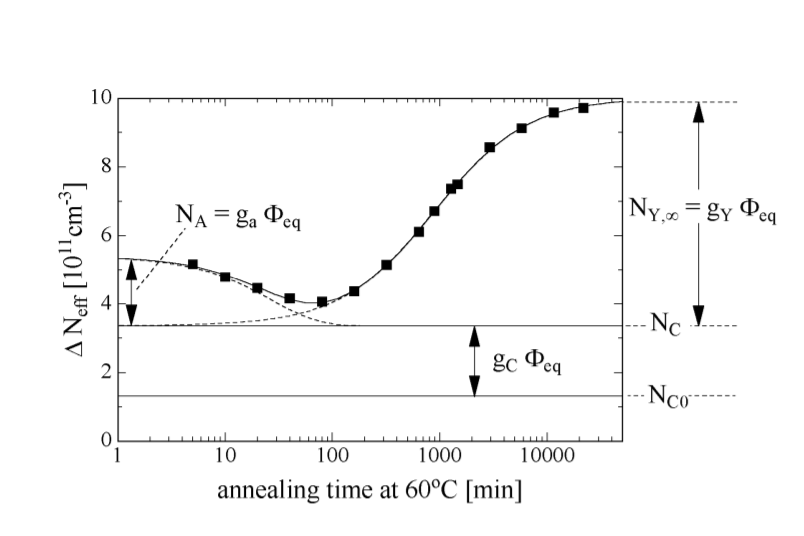
\includegraphics[width=0.95\textwidth]{logos/n_eff_beispiel.PNG}
  \caption{Dotierungskonzentration bei 60°C für eine Bestrahlung mit einer Fluenz
  von $\Phi=\SI{1.4e13}{\per\centi\meter\squared}$ .\cite{moll}}
  \label{fig:n_eff_beispiel}
\end{figure}



\section{Annealing des Leckstroms}
Der Leckstrom beschreibt allgemein einen messbaren Stromfluss über einen als isolierend
angenommenen Weg. Bei Halbleitern ist damit der Strom gemeint, der trotz sperrender
Diode fließt. Dieser entsteht durch die Diffusion von einzelnen Ladungsträgern, welche
in der Realität nicht komplett verhindert werden kann.
Zusätzlich kommt ein Leckstrom durch strahlungsinduzierte Defekte hinzu, welche
Elektronen-Loch-Paare generieren \cite{moll}.
Durch das Annealing kann der Leckstrom somit verringert werden.

Die Fluenz und der durch Strahlung hervor gerufene Leckstrom $\Delta I$ sind
proportional zueinander.


\begin{align}
  \Delta I = \alpha \Phi_{\mathrm{eq}} \cdot V
\end{align}
Hierbei ist $V$ das Volumen des Detektormaterials und $\alpha$ die
sogenannte Schadensrate.
%Der Leckstrom ist vor der Bestrahlung des Sensors
%vernachlässigbar klein im Vergleich zu dem Leckstrom nach der Bestrahlung,
%weshalb $\Delta I$ als Näherung den gesamten Leckstrom beschreibt.

Der Leckstrom vor und nach der Bestrahlung ist temperaturabhängig und wird
beschrieben durch
\begin{align}
  I(T) \propto T^2 \exp{\frac{-E_{\mathrm{g}}}{2 k_{\mathrm{B}}T}} \text{\cite{moll}} \label{eqn:Chilingarov_2013}.
\end{align}
Hier ist $E_{\mathrm{g}}$ die Energie der Bandlücke.

Die Verringerung des Leckstromes durch annealing wird mit der Schadensrate
beschrieben, welche als eine Funktion abhängig von der Zeit und
Temperatur beschrieben wird.\cite{moll}

\begin{align}
  \alpha(t, T) = \underbrace{\alpha_I \cdot \exp{\left(-\frac{t}{\tau_{\mathrm{I}}(T)}\right)}}_{\mathrm{shortterm \: annealing}} + \underbrace{\alpha_{\mathrm{0}}(T) -\beta \cdot \ln{\left(\frac{t}{t_{\mathrm{0}}}\right)}}_{\mathrm{longterm \: annealing}} \text{\label{eqn:damage}}
\end{align}
Mit der Amplitude $\alpha_I$, dem Parameter $\beta$, den in \cite{moll} berechnete Werten für $\alpha_{\mathrm{0}}(T)$, sowie der
temperaturabhängigen Funktion $\tau_{\mathrm{I}}(T)$:
\begin{align}
  &\alpha_{\mathrm{0}}(T) = \SI{-8.9e-17}{\ampere\per\centi\meter} + \SI{4.6e-14}{\ampere\kelvin\per\centi\meter} \cdot \frac{1}{T} \\
  &\tau_{\mathrm{a}}(T) = \frac{1}{k_{0\mathrm{I}}}\exp{\left(\frac{E_{I}}{k_{\mathrm{b}}T}\right)}
\end{align}
Wie für $N_{\mathrm{A}}$ und $N_{\mathrm{Y}}$ ist $k_{0\mathrm{I}}$ ein Frequenzfakor und $E_{I}$ die Aktvierungsenergie.

Anders als das Annealingverhalten der Dotierungskonzentration kann die Schadensrate
bei fortschreitendem annealing nur sinken. Für kurze und
lange Zeiten dominieren wie bei der Dotierungskonzentration unterschiedliche
Terme. Für große Temperaturen und Zeiten würde die Schadensrate kleiner als null
werden. Die Messwerte für kleine $\alpha$ weichen jedoch von dem
theoretischen Verlauf ab und nähern sich einen Wert größer null an. Dies
ist in Abbildung \ref{fig:damage_rates} dargestellt.

\begin{figure}
  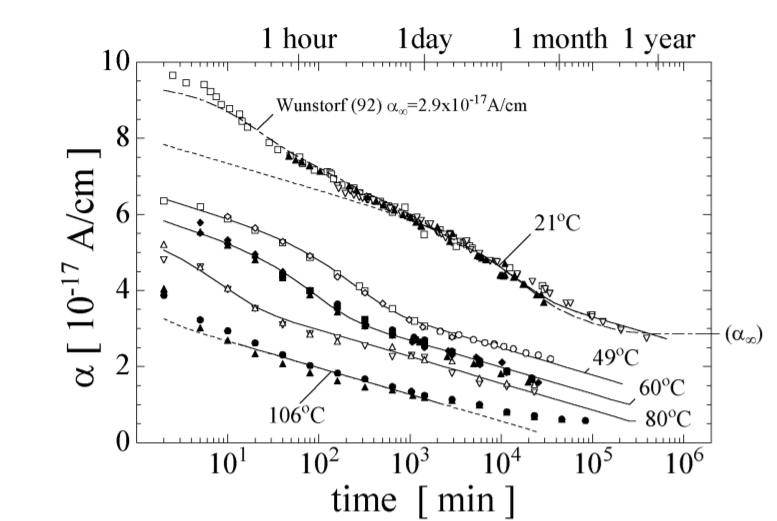
\includegraphics[width=0.9\textwidth]{logos/schadensraten.PNG}
  \caption{Schadensraten für verschiedene konstante Annealingtemperaturen.\cite{moll}}
  \label{fig:damage_rates}
\end{figure}

\chapter{Entwicklung des Programmes zur Berechnung von Annealingeffekten}\label{make}
Die folgenden Unterkapitel beschreiben die Vorgehensweise für die Entwicklung  eines Programmes zur
Berechnung von Annealingeffekten. Das Programm ist in der Programmiersprache Python unter
der Verwendung der \textit{NumPy}, \textit{Matplotlib} und \textit{math} Bibliotheken geschrieben.
\section{Annealingeffekte für konstante Temperaturen}
Zur Überprüfung der Implementation der Funktionen werden
Gleichung \ref{eqn:N_eff} und \ref{eqn:damage}  bei konstanter Temperatur verwendet. In
Abbildung \ref{fig:N_eff} und \ref{fig:damage} sind diese, für $10^5$ Minuten bei einer Temperatur
von $\SI{60}{\celsius}$ und $\SI{80}{\celsius}$  dargestellt.
Für alle Plots werden Fitparameter
einer "WE-25k" Diode aus \cite{moll} genommen und sind in Tabelle \ref{tab:w1} dargestellt. Die verwendeten
Parameter sind beispielhaft gewählt und können gezielt angepasst werden.

%\begin{table}[H]
%\centering
%\caption{Positionen der Photodiode und gemessene Stromstärken}
%\sisetup{table-format=2.1}
%\begin{tabular}{S S S S S S}
%  \toprule
%    \multicolumn{5}{c}{Fitparameter} & \multicolumn{1}{c}{Materialparameter} \\
%    \cmidrule(lr){1-5}\cmidrule(lr){6-6}
%    {$\alpha_{\mathrm{I}}/10^{-17}\, \mathrm{Acm^{-1}}$} & {$\beta/\, /10^{-17}\, \mathrm{Acm^{-18}}$} & {$k_{0\mathrm{I}}/\,10^{13}\mathrm{s^{-1}}$} &
%    {$k_{0\mathrm{a}}/\,10^{13}\mathrm{s^{-1}}$} & {$k_{Y\mathrm{I}}/\,10^{15}\mathrm{s^{-1}}$} & {$E_{\mathrm{I}}/\, \mathrm{eV}$} \\
%    \midrule
%    1 & 1 & 1 & 1 & 1 \\
%    \bottomrule
%  \end{tabular}
%\end{table}

\begin{table}
  \centering
  \caption{Fitparameter der "WE-25k" Diode für die Modellierung von Annealingeffekten }
  \label{tab:w1}
  \begin{tabular}{c c}
    \toprule
    Fitparameter & Wert  \\
    \midrule
        $\alpha_{\mathrm{I}}$  &    1,23 $\cdot$ $  10^{-17}        \mathrm{Acm^{-1}}$    \\
        $\beta $               &    3,07 $\cdot$ $10^{-17}          \mathrm{Acm^{-18}}$     \\
        $N_{\mathrm{C0}}$             &    1,1  $\cdot$            $10^{11}\mathrm{cm^{-3}}$   \\
        $c$                          &    75   $\cdot$             $10^{-14}\mathrm{cm^{-2}}$    \\
        $k_{0\mathrm{I}}$            &    1,2  $\cdot$             $10^{13}\mathrm{s^{-1}}$\\
        $k_{0\mathrm{a}}$           &    2,4  $\cdot$              $10^{13}\mathrm{s^{-1}}$   \\
        $k_{0\mathrm{Y}}$            &    1,5  $\cdot$             $10^{15}\mathrm{s^{-1}}$     \\
        $E_{\mathrm{I}}$                       &    1,11           $\mathrm{eV}$       \\
        $E_{\mathrm{aa}}$                     &    1,09            $\mathrm{eV}$       \\
        $E_{\mathrm{Y}}$                      &    1,33            $\mathrm{eV}$    \\
        $g_{\mathrm{c}}$      &    1,58 $\cdot$                    $10^{-2}\mathrm{cm^{-2}}$           \\
        $g_{\mathrm{a}}$           &    1,59 $\cdot$               $10^{-2}\mathrm{cm^{-2}}$         \\
        $g_{\mathrm{Y}}$          &    4,84 $\cdot$                $10^{-2}\mathrm{cm^{-2}}$      \\
    \bottomrule
  \end{tabular}
\end{table}
Die \textit{introduction rates} und die Fitparameter $N_{\mathrm{C0}}$, $c$, $\alpha_{\mathrm{I}}$ und $\beta $ sind dabei materialabhängig.

\begin{figure}
  \centering
    \includegraphics[width=0.82\textwidth]{build/annealing.PDF}
    \caption{$\Delta N_{\mathrm{eff}}$ einer WE-25k Diode nach einer Bestrahlung mit einer Fluenz von
    $5\cdot 10^{15} \, \mathrm{n_{\mathrm{eq}}/cm^2}$.}
    \label{fig:N_eff}
\end{figure}

\begin{figure}
  \centering
    \includegraphics[width=0.82\textwidth]{build/damage.PDF}
    \caption{Schadensrate einer WE-25k Diode.}
    \label{fig:damage}
\end{figure}

Beide Annealingeffekte stimmen mit dem Verlauf von Abbildung \ref{fig:n_eff_beispiel} und \ref{fig:damage_rates} über ein, was
die korrekte Implementierung der Funktionen \ref{eqn:N_eff} und \ref{eqn:damage}  des Programms
bestätigt.



\section{Annealingeffekte für nicht konstante Temperaturen}{\label{nicht_konstant}}
Die Gleichungen \ref{eqn:N_eff} und \ref{eqn:damage} gehen bei der Berechnung der Annealingeffekte von
einer konstanten Temperatur aus, wodurch diese nicht geeignet sind um $\Delta N_{\mathrm{eff}}$ und $\alpha$ für
Temperaturverläufe zu berechnen, welche deutlich von einer konstanten Temperatur abweichen.


%Werden die selben Gleichungen zur Modellierung von Annealingeffekte für nicht
%konstante Temperaturen verwendet, so kommt es zu deutlichen Abweichungen für
%$\Delta N_{\mathrm{eff}}$ und $\alpha$ im Vergleich zu dem eigentlich erwarteten
%Verhalten nach dem Hamburg-Modell.
In Abbildung \ref{fig:N_eff_ohne} und \ref{fig:damage_ohne} ist das Annealingverhalten
der Dotierungskonzentration und der Schadensrate mit
diesem Ansatz dargestellt.
Das Temperaturprofil wurde während der Bestrahlung
des Sensors "R1" mit Reaktorneutronen in den
"Sandia National Laboratories" aufgenommen.
Weitere Informationen zu dem Sensor und
der Bestrahlungen finden sich in \cite{mareike}.

\begin{figure}
  \centering
    \includegraphics[width=0.82\textwidth]{build/ohnekorrektur.PDF}
    \caption{Dotierungskonzentration des Sensors R1 im Verlauf des Annealings nach einer Bestrahlung mit einer Fluenz von
    $5\cdot 10^{15} \, \mathrm{n_{eq}/cm^2}$.}
    \label{fig:N_eff_ohne}
\end{figure}

\begin{figure}
  \centering
    \includegraphics[width=0.82\textwidth]{build/damageohnekorrektur.PDF}
    \caption{Schadensrate des Sensors R1 im Verlauf des Annealings.}
    \label{fig:damage_ohne}
\end{figure}

%\begin{figure}
%  \centering
%  \begin{subfigure}{0.48\textwidth}
%      \centering
%      \includegraphics[height=0.82\textwidth]{build/ohnekorrektur.PDF}
%  \end{subfigure}
%  \begin{subfigure}{0.48\textwidth}
%      \centering
%      \includegraphics[height=0.82\textwidth]{build/damageohnekorrektur.PDF}
%  \end{subfigure}
%  \caption{Dotierungskonzentration (a) und Schadensrate (b) des Sensors R1 nach einer Bestrahlung mit Fluenz $\Phi_{\mathrm{eq}} = \SI{5e15}{\per\centi\meter\squared}.$}
%\end{figure}
%  \subfigure[]{\includegraphics[width=0.49\textwidth]{build/damageohnekorrektur.PDF}}
%  \caption{Dotierungskonzentration (a) und Schadensrate (b) des Sensors R1 nach einer Bestrahlung mit Fluenz $\Phi_{\mathrm{eq}} = \SI{5e15}{\per\centi\meter\squared}.$}
%  \label{fig:ohnekorrektur}
%\end{figure}

Die Dotierungskonzentration strebt nach dem Hamburger Modell
für unendlich große Zeiten gegen einen konstanten Wert und nimmt nicht mehr
ab.
Der Fehler entsteht, da Gleichung \ref{eqn:N_eff} für jeden
Zeitpunkt eine konstante Temperatur annimmt. Jedoch ist es für Annealingeffekte
relevant die Annealinghistorie zu berücksichtigen.
Das bedeutet, dass $\Delta N_{\mathrm{eff}}$ für große Zeiten abfällt, da die Gleichung über den
gesamten Zeitraum mit den zugehörigen kleinen Temperaturen rechnet. Für
die Schadensrate gilt das gleiche Problem.

Um die Effekte richtig berechnen zu können, muss eine Korrektur in den
Gleichungen vorgenommen werden.
Zunächst wird die Dotierungskonzentration betrachtet. Als Näherung wird über
jeden einzelnen Zeitabschnitt $t_{\mathrm{i}} - t_{\mathrm{i-1}}$ die
Temperatur $(T_{\mathrm{i}} +T_{\mathrm{i-1}})/2$ für das Annealing verwendet.
Da der stable damage keine Temperaturabhängigkeit hat, muss dieser nicht
verändert werden. Für $N_{\mathrm{A}}$ wird nun folgende Näherung
verwendet:

\begin{align}
  &\frac{t_{\mathrm{n}}}{\tau_{\mathrm{a}}(T_{\mathrm{n}})} \rightarrow \sum_{i=0}^n  \frac{t_{\mathrm{i}} - t_{\mathrm{i-1}}}{\tau_{\mathrm{a}}(\frac{T_{\mathrm{i}} +T_{\mathrm{i-1}}}{2})} \:\:\:\: \text{für} \: n>0 \\
\end{align}
Für den Zeitpunkt $t=0$ gilt weiterhin $t_{\mathrm{n}}/(\tau_{\mathrm{a}}(T_{\mathrm{n}})) = 0$.
Durch die Summation der einzelnen Zeitabschnitte mit dem Mittelwert der dazugehörigen
Temperatur kann die gesamte Temperaturkurve beschrieben werden. Für $N_{\mathrm{Y}}$
wird analog die gleiche Korrektur durchgeführt.
In Abbildung \ref{fig:korrektur_N_eff} ist Dotierungskonzentration mit Korrektur dargestellt.


\begin{figure}[!htb]
  \centering
    \includegraphics[width=0.82\textwidth]{build/annealingtdata.PDF}
\caption{$\Delta N_{eff}$ des Sensors R1 mit Korrektur nach einer Bestrahlung mit einer Fluenz von $5\cdot 10^{15} \, \mathrm{n_{eq}/cm^2}$.}
\label{fig:korrektur_N_eff}
\end{figure}



Der Verlauf entspricht nun den Erwartungen, ist aber lediglich als Näherung zu verstehen, da angenommen
wird, dass die Bestrahlung vor dem Annealing stattgefunden hat. Die Sensoren wurden jedoch
während dem Annealing bestrahlt, wodurch ein genaues Berechnen der Annealingeffekte nicht
möglich ist. Für präzisere Ergebnisse sind Informationen über die zeitliche Änderung der Fluenz nötig,
zusätzlich ist die Interaktion zwischen der Fluenz und dem Annealingprozess nicht bekannt.



%Mit der Berücksichtigung
%der einzelnen Temperaturen verzögert sich der Annealingeffekt insgesamt, da anfänglich
%geringe Temperaturen nur wenig zum gesamten Effekt beitragen. Dies wird
%an dem späteren Zeitpunkt des Minimums deutlich.

Eine solche Korrektur kann für den \textit{shortterm annealing} Term der Schadensrate ebenfalls erstellt werden.
Im zweiten Term ist $\alpha_{0}$ temperaturabhängig, aber nicht zeitabhängig,
wodurch der Korrekturansatz hier nicht mehr gelten kann. Um den Ansatz dennoch
verwenden zu können, wird die Zeit des \textit{longterm annealing} mit dem in \cite{moll} vorgeschlagenen
Skalierungsfaktor
\begin{align}
  \Theta(T) =  \exp{\left(-\frac{E_{\mathrm{I}}^*}{k_b}\left(\frac{1}{T}-\frac{1}{T_{\mathrm{ref}}}\right)\right)} \\
\end{align}
versehen, wodurch sich die Formel der Schadensrate  zu
\begin{align}
  &\alpha(t, T) = \alpha_I \cdot \exp{\left(-\frac{t}{\tau_{\mathrm{I}}(T)}\right)} + \alpha_{\mathrm{0}}^{*} -\beta \cdot \ln{\left(\Theta(T) \cdot \frac{t}{t_{\mathrm{0}}}\right)} \\
  \medskip
  \text{mit}\:\: &\alpha^*_{\mathrm{0}}(T) = \SI{-8.9e-17}{\ampere\per\centi\meter} + \SI{4.6e-14}{\ampere\kelvin\per\centi\meter} \cdot \frac{1}{T_{\mathrm{ref}}}
\end{align}
ändert.
Hierbei ist $E_{\mathrm{I}}^*$ eine Aktivierungsenergie und $\alpha^*_{0}$ nun nicht mehr temperaturabhängig,
sondern lediglich abhängig von einer Referenztemperatur $T_{\mathrm{ref}}$. Für konstante Temperaturen
ist diese Gleichung folglich äquivalent zu Gleichung \ref{eqn:damage}, für nicht
konstante Temperaturen ist die resultierende Abweichung im Vergleich zur Korrektur vernachlässigbar.
Nun kann wieder eine Korrektur analog zu den vorherigen eingeführt werden:

\begin{align}
  \Theta(T) \cdot t_{\mathrm{n}} \rightarrow \sum_{i=0}^n   \Theta \left(\frac{T_{\mathrm{i}} +T_{\mathrm{i-1}}}{2}\right) \cdot  (t_{\mathrm{i}} - t_{\mathrm{i-1}})
\end{align}

In Abbildung \ref{fig:korrektur_damage} ist die Schadensrate mit Korrektur
dargestellt.

\begin{figure}
  \centering
    \includegraphics[width=0.82\textwidth]{build/damagekorrektur.PDF}
\caption{Schadensrate des Sensors R1 mit Korrektur.}
\label{fig:korrektur_damage}
\end{figure}
%\begin{figure}
%  \begin{subfigure}[]{\linewidth}
%    \includegraphics[width=0.49\textwidth]{build/damageohnekorrektur.PDF}
%  \end{subfigure}
%  \begin{subfigure}{\linewidth}
%    \includegraphics[width=0.49\textwidth]{build/damagekorrektur.PDF}
%  \end{subfigure}[]
%  %\caption{Schadensrate des Sensors R1 ohne Korrektur (a) und mit Korrektur (b).}
%  %\label{fig:korrektur_damage}
%\end{figure}


%Auch hier zeigt das Verhalten ohne Korrektur klare Abweichungen zu den
%Erwartungen, so kann beispielsweise die Schadensrate mit voranschreitendem Annealing nicht steigen.
Mit Korrektur verhält sich die Schadensrate gemäß den Erwartungen, der stärkste
Effekt ist bei den größten Temperaturen zu sehen, kleine Temperaturen führen hingegen
nur zu minimalen Änderungen.

Mit der Implementierung dieser Korrekturen kann das Programm Annealingeffekte für
beliebige Temperaturverläuft berechnen.



\section{Lineare Interpolation der Temperatur}
Der im vorherigen Abschnitt beschriebene Korrekturansatz verwendet für jedes
Zeitintervall den Mittelwert der Anfangs- und Endtemperatur. Für große
Zeitabschnitte kommt es bei Temperaturprofilen wie bei Sandia also auch zu größeren Abweichungen von der tatsächlichen
Temperatur. Um diesen Fehler gering zu halten, wird das Temperaturprofil
linear interpoliert.
Um die Rechenzeit nicht unnötig zu erhöhen, wird eine Funktion definiert, die sinnvolle
Interpolationsschritte $n$ zwischen zwei Messpunkten abschätzt.
Da große Temperaturen relevanter für das Annealing sind und die Annealingeffekte nicht linear von
der Temperatur abhängig sind, ist es vorteilhaft,
bei den Mittelwerten der Temperaturen möglichst kleine Ungenauigkeiten und somit möglichst viele
Intervalle zu erschaffen. Aus diesem Grund wird die minimale Temperatur $T_{\mathrm{min}}$ des Datensatzes
als Bezugspunkt genommen, wobei die Parameter $y$ und $z$ frei anpassbar sind:

\begin{align*}
  n = \lceil{y \cdot (T-T_{\mathrm{min}})+ z}\rceil \label{eqn:intervall} .
\end{align*}
Die Funktion wächst mit steigenden Temperaturen und gibt die Anzahl auf eine Temperatur $T(t_{\mathrm{i}})$ des
Datensatzes folgenden Intervalle bis zur nächsten Temperatur $T(t_{\mathrm{i+1}})$ an. Der Parameter $z$ bewirkt eine allgemeine Steigerung
der Anzahl an Intervallen, während $y$ die Anzahl basierend auf der zu betrachtenden Temperatur
erhöht.


Für die Zeit und die Temperatur der interpolierten Daten gilt:
\begin{align}
  t_i &= t_{\mathrm{A}} +  \frac{t_{\mathrm{B}}-t_{\mathrm{A}}}{n} \cdot i \\
  T_i &= T_{\mathrm{A}} +  \frac{T_{\mathrm{B}}-T_{\mathrm{A}}}{n} \cdot i \\
  \text{mit}\:\:i &= 1, 2, ..., n
\end{align}

Hierdurch werden lineare und gleich lange Intervalle zwischen den Temperaturen
erzeugt. In den Abbildungen \ref{fig:interpolation_N_eff} und \ref{fig:interpolation_damage} sind die interpolierten Temperaturen und
die daraus berechneten Annealingeffekte dargestellt.

\begin{figure}
    \includegraphics[width=0.82\textwidth]{build/interpolationtdata.PDF}
\caption{$\Delta N_{\mathrm{eff}}$ und zugehörige Interpolierte Temperatur für y = $0,05$ und $z=0,2$.}
\label{fig:interpolation_N_eff}
\end{figure}



\begin{figure}
  \centering
    \includegraphics[width=0.82\textwidth]{build/damage_interpolation.PDF}
\caption{Interpolierte Temperatur für y = $0,05$ und $z=0,2$ und $\alpha$.}
\label{fig:interpolation_damage}
\end{figure}

Die Anzahl der Intervalle der linearen Interpolation steigt gemäß der Funktion \ref{eqn:intervall}
für größer werdende Temperaturen. Durch die Verwendung der Interpolation kommt es zu kleinen Abweichungen im
Vergleich zu einer Berechnung die lediglich die Messpunkte nutzt.
%Da die lineare Interpolation lediglich eine Näherung des Verlaufes der
%Temperaturkurve entspricht, kommt es bei der Aufsummierung der einzelnen Zeitabschnitte
%zu größer werdenden Abweichungen von der eigentlichen Kurve.
Die abweichenden Werte beschreiben
aufgrund der Interpolation einen präziseren Verlauf als der Annealingeffekt des ursprünglichen Datensatzes.
Jedoch beschreibt die lineare Interpolation nur eine Näherung des wahren Temperaturverlaufes.

\section{Berechnung der gesamten Annealinghistorie eines Sensors}
Die hier betrachtete Annealinghistorie setzt sich aus 60 Erwärmungs-und
Abkühlungszyklen des Sensors "P3" zusammen, welche insgesamt $\SI{1800}{\minute}$ entsprechen.
Für den Sensor "P4" werden 39 Zyklen ($\SI{1170}{\minute}$) betrachtet.
Beide wurden von der ${\mathrm{IRRAD}}$ Einrichtung mit $\SI{24}{\giga\eV\per\clight}$ Protonen des Protonen Synchrotrons bestrahlt.
Die Datensätze werden mithilfe eines Python Programmes miteinander Verbunden,
wobei die Zeiten zwischen dem Annealing von einem Zyklus zum nächsten auf null gesetzt werden. Wegen der geringen
Temperaturen nach jeder Abkühlung sind die daraus resultierenden Abweichungen vernachlässigbar.
Für jeden Zyklus wurde bei den Sensoren eine Temperatur von $\SI{60}{\celsius}$ angestrebt.
Mehr Informationen zu den Eigenschaften von P3 und P4 in  \cite{felix}.


In Abbildung \ref{fig:P_3} ist die Schadensrate für die 60 Annealingzyklen,
sowie die experimentell bestimmte Schadensrate dargestellt.

\begin{figure}
  \centering
    \includegraphics[width=0.82\textwidth]{build/damage_ohne_temperatur.PDF}
\caption{Theoretische Schadensrate und gemessene Schadensrate nach 1, 2, 3, 4, 6, 9, 14, 24, 39 und 60 Zyklen .}
\label{fig:P_3}
\end{figure}

Der stufenartige Verlauf der Kurve resultiert aus den Temperaturzyklen.
Es ist eine merkliche Abweichung der experimentellen Messwerte von den theoretischen
Werten erkennbar. Der Sensor "P3" wurde schon vor der Messung unkontrolliert erwärmt, wodurch
die angegebenen Annealingzeiten in Wahrheit größer sind und nicht präzise abgeschätzt werden können. Dies erklärt die
geringe Änderung der einzelnen Messwerte voneinander, welche dem
Verlauf der theoretischen Werte für große Zeiten ähnelt. Die Abweichung der theoretischen
und experimentellen Funktionswerte wird dadurch größer.
Für die Bestimmung der Schadensrate wird das Detektorvolumen und den durch
Strahlung induzierten Leckstrom $\Delta I$ benötigt. Bei der Messung wurde
$\Delta I$ mit dem Leckstrom gleichgesetzt. Dies gilt nur bei einer Temperatur
von $\SI{20}{\celsius}$, bei der Messung des Stroms betrug die tatsächliche Temperatur
$\SI{-2}{\celsius}$. Um dies zu korrigieren wird der Leckstrom gemäß \ref{eqn:Chilingarov_2013}
mit der Temperatur skaliert. Die Energie der Bandlücke und das Volumen des Detektormaterials
unterliegen dabei Unsicherheiten. Zusätzlich haben auch die materialspezifischen Parameter
der theoretischen Messwerte eine gewisse Abweichung zu den tatsächlichen Parametern, da
ein anderer Sensor betrachtet wird.

Die Messung des Sensors "P4" ist in Abbildung \ref{fig:P_4}
dargestellt.

\begin{figure}
  \centering
    \includegraphics[width=0.82\textwidth]{build/damage_P_4.PDF}
\caption{Theoretische Schadensrate und gemessene Schadensrate nach 1, 2, 3, 4, 6, 9, 14, 24 und 39 Zyklen.}
\label{fig:P_4}
\end{figure}

Die Abweichungen sind in dieser Messreihe noch deutlicher. Neben den Fehlerquellen die
für den Sensor "P3" aufgezählt wurden, ist "P4" zusätzlich nicht vollständig depletiert.
Für die Bestimmung des aktiven Volumens zur Berechnung der Schadensrate wurde ein vollständig
depletierter Sensor angenommen. Das tatsächliche aktive Volumen des Detektors ist somit kleiner, wodurch sich auch
die gemessene Schadensrate verringert.
Um diesen Effekt berücksichtigen zu können, müsste das Depletierte Volumen
beispielweise über Ladungssammlungseffizienz (CCE) Messungen bestimmt werden.
%Die Funktion \ref{eqn:damage} kann solche Effekte nicht berücksichtigen.

\input{content/04_interface.tex}
\chapter{Zusammenfassung}
Im Zuge dieser Arbeit wurde ein Programm entwickelt, dass
die Dotierungskonzentration und die Schadensrate während dem
Annealing einer bestrahlten Diode
auf der Grundlage des Hamburger Modells beschreibt.

Durch beliebig viele Interpolationsintervalle im Temperaturprofil kann die entstehende Abweichung des
Korrekturansatzes klein gehalten werden.
%Die Näherung für beliebige
%Temperaturverläufe verursacht für hinreichend viele Interpolationsintervalle
%vernachlässigbar kleine Fehler.

Für große Annealingzeiten beschreibt Gleichung \ref{eqn:damage} nicht mehr die tatsächliche Schadensrate, wodurch das Programm,
welches auf dieser Gleichung basiert, dies ebenfalls nicht kann. Abweichungen
von dem Hamburger Modell werden jedoch erst nach
einer Annealingzeit von mehr als $t=\SI{e4}{\minute}$ bei $\SI{80}{\celsius}$ erreicht (siehe
\ref{fig:damage_rates}). Für solche Werte liegt
die Dotierungskonzentration bereits nahe am Sättigungswert.

%Die Anwendbarkeit des Modells zur Berechnung der Schadensrate ist
%beschränkt, so würden große Annealingzeiten und Temperaturen ($\alpha < \SI{1.5e-17}{\ampere\per\centi\meter}$) zu Abweichungen
%zwischen Modell und Realität führen. Solche Werte werden jedoch erst nach
%einer Annealingzeit von mehr als $t=\SI{e4}{\minute}$ bei $\SI{80}{\celsius}$ erreicht (siehe
%\ref{fig:damage_rates}), wofür
%die Dotierungskonzentration bereits nahe am Sättigungswert liegt.
%versagt für kleine Schadensraten $\alpha < \SI{1.5e-17}{\ampere\per\centi\meter}$,
%da diese nicht beliebig gering werden können. Solche Werte werden jedoch erst nach
%einer Annealingzeit von mehr als $t=\SI{1e4}{\minute}$ bei $\SI{80}{\celsius}$ erreicht, wofür
%die Dotierungskonzentration bereits nahe am Sättigungswert liegt.

%Die Verbindung von Datensätzen und die Anknüpfung der einzelnen Zeitstempel der
%Textdateien funktioniert.
%Abweichungen von experimentellen Daten führen zu vernachlässigbar kleinen Ungenauigkeiten, da das Annealing
%nach einem Abkühlungszyklus selbst über große Zeiträume irrelevant im Vergleich zu
%den Erwärmungszyklen ist.

Abweichungen von experimentellen Daten sind durch systematische Unsicherheiten der Messdaten
zu erklären. Unvollständige Depletion des Sensors, vorheriges Annealing über einen
unbekannten Zeitraum und Unsicherheiten in der Temperaturskalierung des Leckstroms sind dabei die Hauptursachen.

Es wurde ein Interface erstellt, dass das Modell nutzt um die Schadensrate und die Dotierungskonzentration
für beliebige Fluenzen, Temperaturen und
Zeiten vorherzusagen. Die dargestellten Werte entsprechen den genauen Funktionswerten
der Funktionen \ref{eqn:N_eff} und \ref{eqn:damage}, da keine Näherungen nötig sind.

Das erstellte Programm kann nur Annealingeffekte mit konstanter Fluenz bestimmen.
Die präzise Modellierung des Annealingverhaltens während der Bestrahlung ist
hiermit nicht möglich. Aus diesem Grund ist eine Aussage über die Genauigkeit der
Modellierung der Annealingeffekte für das Temperaturprofil des in Sandia bestrahlten Sensors nicht möglich.

%dieses während der Bestrahlung aufgenommen wurde. Um nicht konstante Fluenzen
%betrachten zu können, müssen Annahmen über den zeitlichen Verlauf der Bestrahlung getroffen
%werden, welche für das hier betrachtete Temperaturprofil nicht bekannt sind.
%Zudem ist die Wechselwirkung der Bestrahlung und dem zeitgleichen Annealing unklar.
%Das erstellte Programm kann nur Annealingeffekte mit konstanter Fluenz
%bestimmen. Die präzise Modellierung des Annealingverhaltens während der Bestrahlung
%ist hiermit nicht möglich.
%Aus diesem Grund ist eine Aussage über die Genauigkeit der Modellierung der
%Annealingeffekte für das Temperaturprofil aus Sandia nicht möglich.


%Anders als die Temperaturen, die mit einem Zeitabschnitt
%assoziiert werden, treten die Fluenzen in der Dotierungskonzentration
%unabhängig von der Zeit auf, weshalb eine andere Herangehensweise nötig ist.


\appendix
% Hier beginnt der Anhang, nummeriert in lateinischen Buchstaben
%\chapter{Ein Anhangskapitel}

Hier könnte ein Anhang stehen, falls Sie z.\,B.\ Code, Konstruktionszeichnungen oder Ähnliches mit in die Arbeit bringen wollen.
Im Normalfall stehen jedoch alle Ihre Resultate im Hauptteil der Bachelorarbeit und ein Anhang ist überflüssig.


\backmatter
\printbibliography

\cleardoublepage
\thispagestyle{empty}
\section*{Danksagung}

An dieser Stelle möchte ich mich bei all denjenigen bedanken, die mich während
der Anfertigung meiner Bachelorarbeit unterstützt haben.

Mein Dank gebührt Herrn Professor Dr. Kevin Kröninger, der es mir ermöglicht hat
meine Bachelorarbeit an seinem Lehrstuhl zu schreiben.
Ebenso möchte ich mich bei Herrn Dr. Jens Weingarten, sowie den Mitgliedern der
Detektor Upgrade Abteilung für die konstruktive Kritik und den hilfreichen Anregungen bedanken.

Ein besonderer Dank gilt meinem Betreuer Felix Wizemann, der mir
mein Bachelorthema ermöglichte und mich mit viel Engagement
während meiner Arbeit begleitet hat. Dank seiner Expertise konnte er mich immer wieder in meiner
Recherche und bei meinen Fragen unterstützen.

Professor Dr. Dr. Wolfgang Rhode danke ich für die Übernahme der Zweitkorrektur. 

Auch möchte ich mich bei Jan Lukas Späh, Nils Breer und Michael Windau bedanken, für
den regen fachlichen Austausch in unserem Büro.

Zuletzt möchte ich mich bei meiner Familie für den motivierenden Beistand
während meines gesamten Studiums bedanken.

\cleardoublepage
\thispagestyle{empty}
\section*{Eidesstattliche Versicherung}
Ich versichere hiermit an Eides statt, dass ich die vorliegende Abschlussarbeit mit dem Titel \enquote{\thetitle} selbstständig und ohne unzulässige fremde Hilfe erbracht habe.
Ich habe keine anderen als die angegebenen Quellen und Hilfsmittel benutzt, sowie wörtliche und sinngemäße Zitate kenntlich gemacht. 
Die Arbeit hat in gleicher oder ähnlicher Form noch keiner Prüfungsbehörde vorgelegen.

\vspace*{1cm}\noindent
\begin{center}
  \begin{tabular}{@{}p{0.4\textwidth}@{\hspace{0.15\textwidth}}p{0.4\textwidth}@{}}
  \rule{\linewidth}{0.25pt}& \rule{\linewidth}{0.25pt}\\
  Ort, Datum & Unterschrift
  \end{tabular}
\end{center}

\subsection*{Belehrung}
Wer vorsätzlich gegen eine die Täuschung über Prüfungsleistungen betreffende Regelung einer Hochschulprüfungsordnung verstößt, handelt ordnungswidrig.
Die Ordnungswidrigkeit kann mit einer Geldbuße von bis zu \SI[round-mode=places, round-precision=2]{50000}{€} geahndet werden. 
Zuständige Verwaltungsbehörde für die Verfolgung und Ahndung von Ordnungswidrigkeiten ist der Kanzler/die Kanzlerin der Technischen Universität Dortmund. 
Im Falle eines mehrfachen oder sonstigen schwerwiegenden Täuschungsversuches kann der Prüfling zudem exmatrikuliert werden \mbox{(\S\,63 Abs. 5 Hochschulgesetz --HG--).}

Die Abgabe einer falschen Versicherung an Eides statt wird mit Freiheitsstrafe bis zu 3 Jahren oder mit Geldstrafe bestraft.

Die Technische Universität Dortmund wird ggf.\ elektronische Vergleichswerkzeuge (wie z.\,B.\ die Software \enquote{turnitin}) zur Überprüfung von Ordnungswidrigkeiten in Prüfungsverfahren nutzen. \\[\baselineskip]

\noindent Die oben stehende Belehrung habe ich zur Kenntnis genommen.\\[1cm]
\begin{center}
\begin{tabular}{@{}p{0.4\textwidth}@{\hspace{0.15\textwidth}}p{0.4\textwidth}@{}}
\rule{\linewidth}{0.25pt}& \rule{\linewidth}{0.25pt}\\
Ort, Datum & Unterschrift
\end{tabular}
\end{center}

\end{document}
